\section{Theory}

The basic principles of optical tweezers and the theory for further calculations is described in this section.\\

\subsection{Optical trapping}

To understand the working principle of optical tweezers we consider a spherical dielectric particle, a bead, in a coherent light beam with a symmetrical intensity gradient such as in figure \ref{fig_optic_trap_1}. The light beam will exert a force on the bead in the direction of the highest light intensity of the gradient. To understand this, we need to consider two situations. 

For the situation in which the dimensions of the bead are much greater than the wavelength of the light we can apply straight forward ray optics. In the situation where the size of the bead is much smaller than the wavelength we can approximate the bead as a dipole that feels Lorentz force due to a gradient in the electric field.

For the situation where the dimensions of the bead are much larger than the wavelength of the light beam, we consider that photons can exert a radiation force on the bead. This force is a result of the momentum that photons carry  and will be directly proportional to the light intensity. We now consider two rays of light that reach the bead symmetrical with respect to its centre. Due to the bead's spherical symmetric shape, the light rays will be refracted by the dielectric particle at the same rate, but in opposite directions (see figure \ref{fig_optic_trap_1}). Both light rays will, given the change in direction of the light and the third law of Newton, exert a force on the bead. The light ray with the higher intensity will, however, exert a larger force. If the intensity gradient is larger in the centre of the light beam, such as in figure \ref{fig_optic_trap_1}, this would lead to a net force pointing in the direction of the symmetry axis of the light beam. This force would trap the bead to the optical axis.
In the case of a beam of light being focussed such as in figure \ref{fig_optic_trap_2}, the bead would not only be trapped in the direction perpendicular to the beam axis, but also in the direction of the axis. This is also a result of the change of the refraction of light exerting a force on the bead (see figure \ref{fig_optic_trap_2}). However, to light scattering, the bead is in the axial direction trapped slight behind the waist of the light beam.\cite{shaevitz} 

\begin{figure}[h!]
    \begin{subfigure}{.45\textwidth}
    	\centering
    	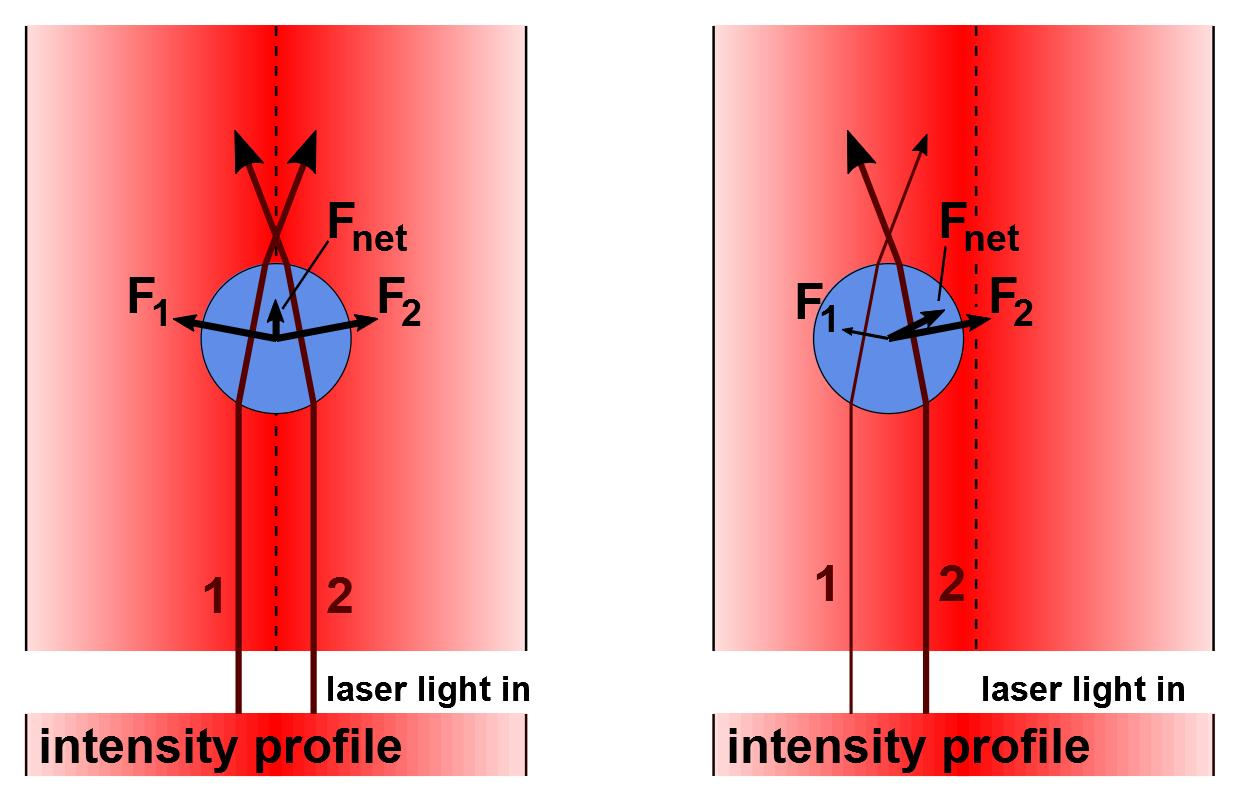
\includegraphics[width=0.9\linewidth,keepaspectratio]{figures/Optical_trap_unfocused.jpg}
    	\caption{ Schematic diagram of the ray optics explanation for optical trapping (unfocused laser). The intensity profile of the light beam is symmetric around the centre. When the bead is displaced from the beam center (right image), the net force is towards the centre due to a larger momentum change of more intense light in closer to the centre. The net force is zero in the horizontal direction when the bead is placed in the centre of the beam. }
    	\label{fig_optic_trap_1}
	\end{subfigure} %
	\hfill
	\begin{subfigure}{0.45\textwidth}
		\centering
		\includegraphics[width=0.9\linewidth,keepaspectratio]{figures/Optical_trap_focused.jpg}
    	\caption{Schematic diagram of the ray optics explanation for optical trapping (focused laser). The light beam is now focussed. Due to the angle of incoming light, the momentum change of the light causes a net force points towards the focus. The equilibrium position is slightly behind the focus to compensate for the light scattering force. }
    	\label{fig_optic_trap_2}
	\end{subfigure}
	\caption{Both figures were taken from Wikipedia \cite{wikipedia}.}
\end{figure}

In the situation where the dimensions of the bead are much smaller of than the wavelength of the light beam, we approximate the bead as a perfect dipole. According to Shaevitz (2006) , if we also consider the laser to have a Gaussian intensity profile in the plane perpendicular to propagation, the Lorentz Force is given by:


\begin{equation}
	F  =  (p \cdot \nabla)E + \frac{1}{c} \frac{d \: p}{dt} \times B
\end{equation}

Where $ p = \alpha E $ is the dipole field, $\alpha $ is the polarizability, $E$ the electric field induced by the light and $B$ the magnetic field induced by the light. Optical traps are typically used with a continuous wave (CW) laser such that $ \frac{\partial}{\partial t}(E \times B) = 0 $ . In this case the magnitude of the time-averaged force in the direction of the optical axis becomes \cite{shaevitz}:

\begin{equation}
	\big \langle F \big \rangle  = \frac{ \alpha }{2} \nabla \big \langle E^2 \big \rangle
\end{equation}

Most optical trapping and also the experiment in this report includes beads with the same order of magnitude dimensions as the wavelength of the light beam. The physics of such a system is complicated and somewhat in between the cases explained above. This comprehensive theory will not be discussed in this report. However, from the latter derivations we can conclude that the trapping force is directly proportional with the laser intensity. \

\subsection{Trap constant derivation}
\label{trap_constant}
\
According to Shaevitz (2006), 'for small motions of a bead near the centre of an optical trap, the forces acting on the bead approximate a zero rest–length, linear spring at the trapping centre.' Therefore, for small motions of the bead, the stored energy in the optical 'spring' is $1/2 k_{trap} \langle x^2 \rangle $ with $k_{trap}$ a constant defining the strength of the optical trap and $ \langle x^2 \rangle $ the variance in the motion. According to the equipartition theory, the energy of the Brownian motion of a particle is given by $\frac{1}{2} k_b T $ with $ k_b $ the Boltzmann constant and $T$ the temperature.\cite{shaevitz} Equating the two energies yields:

\begin{equation}
	\label{eq_k_trap}
	k_{trap} = \frac{k_B T}{ \langle x^2 \rangle}
\end{equation}

From this we can conclude that by following the position of the bead over time, it is possible to find the the value of $k_{trap}$. 

\\

\begin{wrapfigure}{r}{0.5\textwidth}
    \centering
    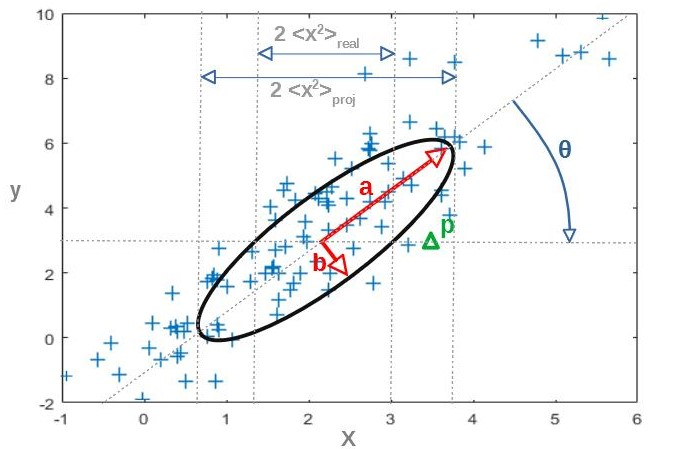
\includegraphics[width=0.45\textwidth,keepaspectratio]{figures/ellips.jpg}
    \caption{Schematic diagram of a data set with a bivariate gaussian distribution. The ellipse represents the variance of the distribution with it's semi-major and semi-minor axis $a$ and $b$. $\theta$ represents the angle between $a$ and line from the centre of the ellipse to an arbitrary point $p$. $\langle x^2 \rangle _{real}$ and $\langle x^2 \rangle _{proj}$ represent respectively the real variance in the x-direction and the projection of the variance ellipse on the x-axis.}
    \label{fig_ellipse}
\end{wrapfigure}


In the latter definition of $k_{trap}$, the 3 dimensions of real life are not taken into account. For the experiments in this report we only consider 2-dimensional images in the plane perpendicular to the propagation direction of the laser beam. This plane will in this report be addressed as the plane of interest, POI. For the POI we can consider two definitions for $k_{trap}$. We define $k_{trap,r}$ as the 'average' trap constant and is calculated using only the motion of the bead in the radial direction. $k_{trap,r}$ gives a good indication of the force in any arbitrary direction in the POI. It does, however, ignore the shape of the probability distribution of the bead. In the case where the potential well would be elongated such as in figure \ref{fig_ellipse}, the values for $ \langle x^2 \rangle $ and therefore also $k_{trap}$ can differ depending on the direction. We define the trap constant in an arbitrary direction as $k_{trap,i}$. Note that this is defined as a line in the POI which cuts the expectation value of the bead. To find the value for $k_{trap,i}$ we first realize that for realistic laser beams that are used for optical trapping, we expect a 2-dimensional gaussian intensity profile in the POI \cite{shaevitz}. The shape of this gaussian profile can be described by a 2 dimensional covariance matrix. The iso-contours and therefore also the variance for such 2-dimensional gaussians are ellipses with their centre at the expectation value \cite{chuong} (see figure \ref{fig_ellipse}. According to Rojas (2009), the eigenvectors of the covariance matrix point in the direction of the axis of an ellipse describing the variance in the POI. The largest of the two eigenvectors, $\vec{v}_1$, will point in the direction of the major axis and the smallest eigenvector, $\vec{v}_2$, in the direction of the minor axis. The magnitude of the semi-major axis and semi-minor axis, $a$ and $b$ respectively, are given by the eigenvalues corresponding to the eigenvectors.\cite{rojas} 

In order to find the variance in any arbitrary direction in the POI,  $ \langle x_i^2 \rangle$, we use the formula for an ellipse in polar coordinates:
\label{alternate_method}

\begin{equation}
	 \langle x_i^2 \rangle ( \theta ) = \frac{a \: b}{\sqrt{( b \: cos\theta)^2 + (a \: sin\theta )^2}}
\end{equation}

Where $\theta$ corresponds to the angle of the direction of interest with respect to the major axis and the ellipse centre as origin. (see figure \ref{fig_ellipse}) \
Note that the latter definition of the variance is different than just projecting each point on an axis and subsequently calculating the variance. The difference between the two methods is clearly visible in figure \ref{fig_ellipse} where $\langle x^2 \rangle _{real}$ is much smaller than $\langle x^2 \rangle _{proj}$. We can conclude from this, that when the position distribution is not symmetrical in the x- and y-direction, calculation of $k_{trap,x}$ or $k_{trap,y}$ without taking into account the covariance could give inaccurate results. Using equation \ref{eq_k_trap} with the value for $  \langle x_i^2 \rangle $ should yield better values for $k_{trap,i}$.


\subsection{Error calculation}

For this report, since we are not fully acquainted with the set-up and the corresponding error, when no error is specified the error is estimated to be half of the finest scale. For example for a size of 1.34 meter, the error would be 0.005 meter.

If $Y$ is a variable which is a function of $A$,$B$,$C$, ... Then the error of $Y$, $u_Y$, is given by equation \ref{eq_error}.

\begin{equation}
	\label{eq_error}
	u_Y = \sqrt{\left(u_A \frac{\partial Y}{\partial A}\right)^2 + \left(u_B \frac{\partial Y}{\partial B}\right)^2 + \left(u_C \frac{\partial Y}{\partial C}\right)^2 + ...}
\end{equation}

Using the latter equation we find that the error in the average position, $u_{\bar{x}}$ is given by:

\begin{equation}
	\label{eq_u_mean}
	u_{\bar{x}} =  \frac{ \sqrt{ \sum_{i=1}^n u_{x_i}^2}}{n}
\end{equation}

Since $ \langle x^2 \rangle $ is given by the average of the squared of the distance to the average position we find that the error in the variance, $u_{ \langle x^2 \rangle } $ is given by:

\begin{equation}
	\label{eq_u_var}
	u_{ \langle x^2 \rangle }=  \sqrt{ \frac{ 4 \: \sum_{i=1}^n    \left( u_{\bar{x}}^2 + u_{x_i}^2 \right) \left( \bar{x} - x_i \right)^2}{n^2}}
\end{equation}

For large values of $n$ we can neglect the $ u_{\bar{x}}^2$ term. Therefore we find:

\begin{equation}
	\label{eq_u_var_approx}
	u_{ \langle x^2 \rangle } \approx  \sqrt{ \frac{ 4 \: \sum_{i=1}^n    u_{x_i}^2  \left( \bar{x} - x_i \right)^2}{n^2}}
\end{equation}

If $ u_{x_i}$ is constant we can rewrite this as:

\begin{equation}
	u_{ \langle x^2 \rangle } \approx  \sqrt{  4 \:     u_{x_i}^2  \langle x^2 \rangle }
	\label{eq_u_var_constant}
\end{equation}



Using equation \ref{eq_k_trap} in equation \ref{eq_error} we find that the error in the trap constant, $u_{k_{trap}}$, is given by:

\begin{equation}
	\label{eq_u_k}
	u_{k_{trap}} = \frac{u_{ \langle x^2 \rangle}k_B T}{ \langle x^2 \rangle ^2}
\end{equation}

In the case of a constant value of $ u_{x_i}$ we can use equation \ref{eq_u_var_constant} to find that:

\begin{equation}
	u_{k_{trap}} = 2 \: u_{x_i} k_B T  \langle x^2 \rangle ^{- \frac{3}{2}}
	\label{eq_u_k_constant}
\end{equation}

Using equation \ref{eq_k_trap} we can rewrite this as:

\begin{equation}
	\label{eq_u_k_constant_}
	u_{k_{trap}} = 2 \: u_{x_i} (k_B T)^{-\frac{1}{2}}  k_{trap} ^{\frac{3}{2}}
\end{equation}





